\documentclass[12pt]{article}

\usepackage[margin=1in]{geometry}
\usepackage{amsmath,amsthm,amssymb}
\usepackage{fancyhdr}
\usepackage[small,compact]{titlesec}
\usepackage{float}

\lhead{Erich Menge}
\chead{\classnameandsection}
\rhead{\homeworktitle}

\pagestyle{fancy}

\newcommand{\sethomeworknumber}[1]{
  \newcommand{\homeworktitle}{Homework #1}
}

\newcommand{\N}{\mathbb{N}}
\newcommand{\Z}{\mathbb{Z}}
\newcommand{\homeworkheader}[1]{
  \title{\vspace{2in}\homeworktitle}
  \author{Erich Menge (X.500: menge053, Student ID: 4624713) \\
  #1}
  \maketitle
  \newpage
}

\newenvironment{problem}[1]{
  \ignorespaces
  \section*{Problem #1}
}{
  \ignorespacesafterend
}

\newenvironment{solution}{
  \ignorespaces
  \subsection*{Solution}
}{
  \ignorespacesafterend
}

\newcommand{\classnameandsection}{CSCI 4011 Formal Languages And Automata Theory Section 3}


\sethomeworknumber{3}

\begin{document}
\homeworkheader{\classnameandsection}

\begin{problem}{8.4}
  \begin{solution}
    \begin{enumerate}
      \item Alternative 1 is clustered, cannot be constructed.\\
      \item
        \tuple{11, (1,1)},
        \tuple{12, (1,2)},
        \tuple{18, (1,3)},
        \tuple{19, (2,1)},
        \tuple{19, (2,2)}
      Unclustered, order not significant.\\
      \item
        \tuple{11, (1,1)},
        \tuple{12, (1,2)},
        \tuple{18, (1,3)},
        \tuple{19, (2,1), (2,2) }
      Unclustered, order not significant.\\
      \item 11, 19. Clustered, order is important.\\
      \item
        \tuple{11, (1,1)}, \tuple{19, (2,1)}  Clustered, order is important.\\
      \item
        \tuple{11, (1,1)}, \tuple{19, (2,1), (2,2)}  Clustered, order is important.\\
      \item Alternative 1 is clustered, can't be constructed. \\
      \item
        \tuple{1.8, (1,1)},
        \tuple{2.0, (1,2)},
        \tuple{3.4, (1,3)},
        \tuple{3.2, (2,1)},
        \tuple{3.8, (2,2)}.
        Order is not significant.\\
      \item
        \tuple{1.8, (1,1)},
        \tuple{2.0, (1,2)},
        \tuple{3.4, (1,3)},
        \tuple{3.2, (2,1)},
        \tuple{3.8, (2,2)}.
        Order is not significant.\\
      \item Can't be constructed. GPA is out of order and clusters require order.\\
      \item Can't be constructed. GPA is out of order and clusters require order.\\
      \item Can't be constructed. GPA is out of order and clusters require order.
    \end{enumerate}
  \end{solution}
\end{problem}

\begin{problem}{8.6}
  \begin{solution}
    \begin{figure}[H]
      \centering
      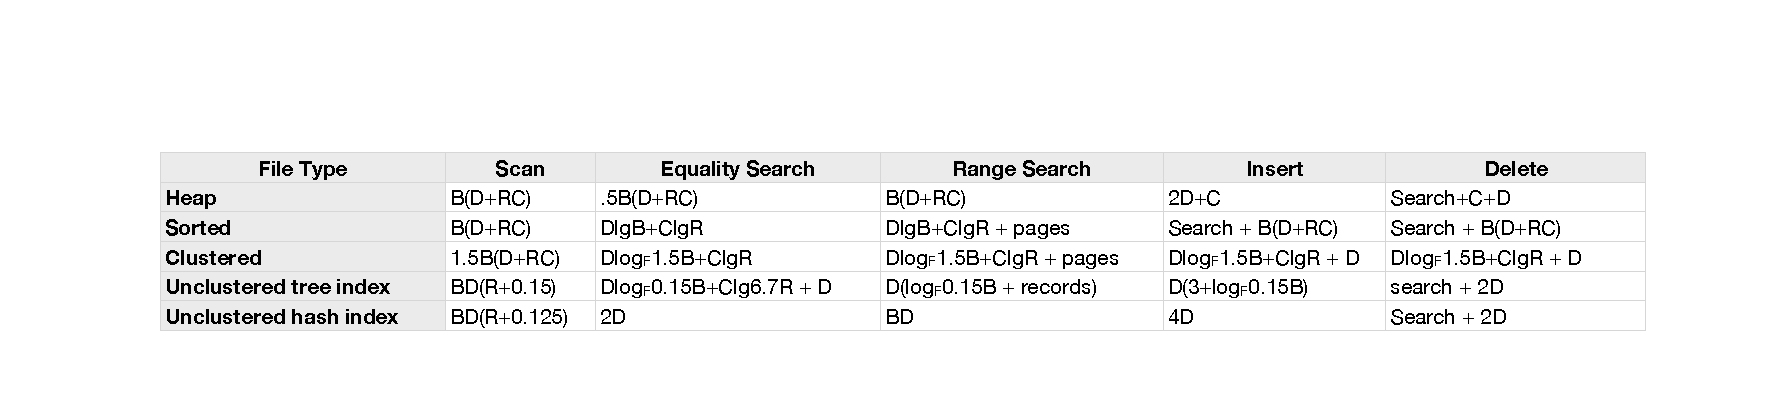
\includegraphics[scale=0.65]{problem_8_6.pdf}
    \end{figure}
  \end{solution}
\end{problem}

\begin{problem}{8.10 parts 2,3 and 4}
  \begin{solution}
    2. Change did for sequential employees (id).\\
    3. Updating age for that same group of employees.\\
    4. Update salary based on DID.
  \end{solution}
\end{problem}

\begin{problem}{12.2}
  \begin{solution}
    \begin{enumerate}
      \item Sorted. \\
      \item Linear hash.\\
      \item B+ Tree index.\\
      \item Sorted file.
    \end{enumerate}
  \end{solution}
\end{problem}

\begin{problem}{12.4}
\end{problem}

\begin{problem}{12.6}
\end{problem}


\end{document}
